\documentclass[article]{xmosmodern}

\includeonly{dsc-software-guide-pwm,dsc-software-guide-qei,dsc-software-guide-adc,dsc-software-guide-hsi,dsc-software-guide-apps,dsc-software-guide-blocks,dsc-software-guide-sdram,dsc-software-guide-display,dsc-software-guide-comms-low,dsc-software-guide-comms-high}

\start

\title{Motor Control Platform Software Guide}
\version{0.13}
\yearmonthday{2011}{02}{09}
\author{Paul Hampson \& Corin Rathbone}

\maketitle

\section*{Release History}

\begin{small}
\renewcommand{\arraystretch}{1.25}
\begin{tabular}{| p{20mm} | p{12mm} | p{88mm}|}
\hline
\textbf{Date} & \textbf{Release} & \textbf{Comment} \\
\hline
2011-02-XX & 1.0 & First release \\
\hline
\end{tabular}
\end{small}

\clearpage

\section{Introduction}
The XMOS motor control development platform is provided with a software framework and example control loop. This document provides information relating to the structure, implementation and use of the software modules that are specific to the motor control development platform.

For information on the XMOS Motor Control Development Platform hardware please see the Motor Control Platform Hardware Manual.

\section{Software Modules}
The provided framework consists of a number of modules that provide functions that combined to provide an integrated control system. The provided application utilises modules that provide the following:

\begin{itemize}
\item Pulse Width Modulation (PWM)
\item Quadrature Encoder Interface (QEI)
\item Analogue to Digital Converter (ADC) Interface
\item Hall Sensor Interface
\item SDRAM Interface
\item Display \& Shared IO Interface
\item Low Level Communications Interfaces (CAN and Ethernet)
\item Application Level Communications (Control And Logging Interfaces)
\item Computation blocks library
\end{itemize}

In contrast to a typical microcontroller, hardware interfaces that are implemented on XMOS devices are all described in software. This gives the developer the flexibility to implement or customise any interface they require. This gives designers wider options when selecting the ADC's or PWM schemes that are required for the solution that is being developed.

Each of the modules is discussed in detail in the sections below.

The modules listed above comprise of one or more threads. The architecture of the threads is shown in the figure \ref{fig_ThreadDiag}. 

\begin{figure}[p]
\begin{center}
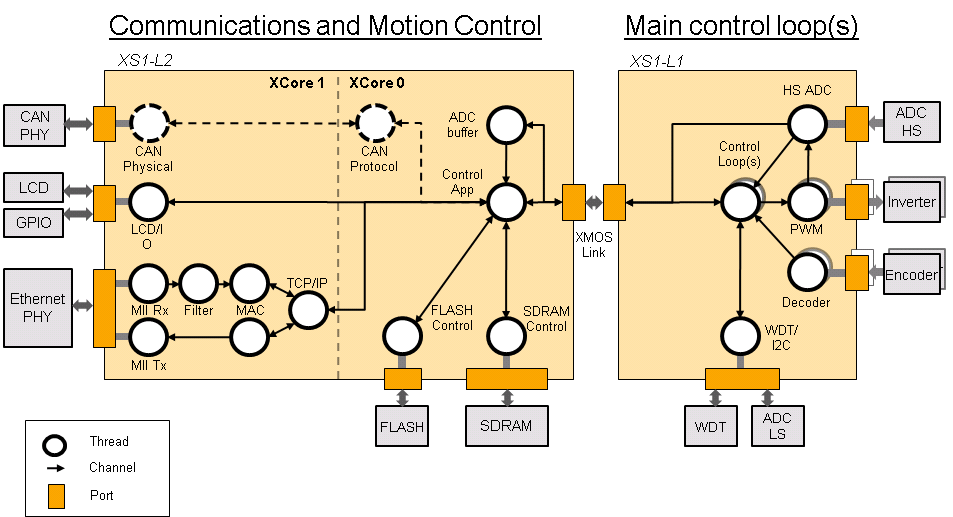
\includegraphics[angle=90,height=0.9\textheight]{images/threadDiag.png}
\caption{Motor Control Platform Thread Diagram}
\label{fig_ThreadDiag}
\end{center}
\end{figure}

\section{Pulse Width Modulation}
The PWM driver code is written using a `client server' model. The client functions are designed to be run from either the main control loop or a separate thread that sits between the control loop and the PWM server thread (dependant on timing constraints defined by the speed of the control loop).

The PWM implementation is centre synchronised. This means that the output is of the form shown in figure \ref{fig_PwmOutputExample}

\begin{figure}[h]
\begin{center}
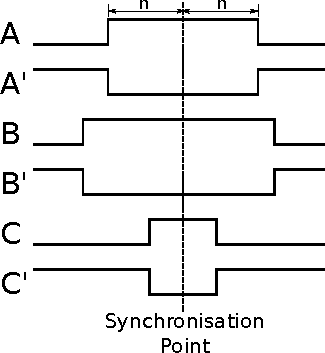
\includegraphics{images/pwmFig.pdf}
\caption{Centrally Synchronised PWM}
\label{fig_PwmOutputExample}
\end{center}
\end{figure}


\subsection{Configuration}
The PWM module has three modes of operation defined, plus a number of other options. The modes are defined in \verb=dsc_config.h= that is part of the application code. 

\subsubsection{PWM Modes}
The PWM operation mode can be one of three of the following options:

\begin{itemize}
\item \verb=PWM_INV_MODE= - This operates a three leg 180 degree inverter by ensuring that the HI and LO sides of the inverter are switched in a complementary manner
\item \verb=PWM_NOINV_MODE= - Simple three channel PWM that operates three channels as above without the inversion
\item \verb=PWM_BLDC_MODE= - Basic BLDC commutation mode operates a three leg inverter by switching the HI side and then applying PWM to the low side of the inverter to achieve simple commutation
\end{itemize}

\subsubsection{Dead Time}
The dead time for \verb=PWM_INV_MODE= is defined using the \verb=PWM_DEAD_TIME= configuration. This is in units of 10ns when using the default reference clock of 100MHz.

\subsubsection{PWM Resolution}
PWM resolution is defined using \verb=PWM_MAX_VALUE=. The value defined here sets the frequency of the PWM. The relationship between \verb=PWM_MAX_VALUE=, \verb=XS1_TIMER_HZ= and PWM frequency ($PWM\_FREQ$) is defined in equation \ref{eqn_PwmFreq}. \verb=XS1_TIMER_HZ= is defined at compile time by the \verb=ReferenceFrequency= identifier in the project XN file. By default this reference frequency is 100MHz so \verb=XS1_TIMER_HZ= would have a value of 100,000,000.

\begin{equation}\label{eqn_PwmFreq}
PWM\_FREQ = \frac{XS1\_TIMER\_HZ}{PWM\_MAX\_VAL} 
\end{equation}

So with an example value of \verb=PWM_MAX_VALUE= being 4096 (12 bit resolution), the \verb=PWM_FREQ= will be 24,414Hz.

\subsubsection{Locking the ADC trigger to PWM}
In some implementations it is desirable to lock the ADC conversion trigger to the PWM. This allows the system to sample the ADC at a specific point in the PWM period (such as when the lower leg is guaranteed to be on). This is enabled using the \verb=LOCK_ADC_TO_PWM= definition.

\subsubsection{Default PWM Configuration}
The default configuration for the demonstration application is as follows. 

\begin{lstlisting}
#define PWM_INV_MODE 1
#define PWM_DEAD_TIME 10
#define PWM_MAX_VALUE 4096
#define LOCK_ADC_TO_PWM 1
\end{lstlisting}

\subsection{PWM Server Usage}
The usage for each mode is described below. The PWM server needs to be instantiated on the same core as the PWM client. The following is required to be included.

\begin{lstlisting}
#include "pwm_service.h"
\end{lstlisting}

\subsubsection{Inverter Mode}
To instantiate the PWM service the function described in the listing below needs to be called for the \verb=PWM_INV_MODE= and \verb=LOCK_ADC_TO_PWM= combination.

\begin{lstlisting}
void do_pwm( chanend c_pwm, chanend c_adc_trig, 
	in port dummy_port, 
	buffered out port:32 p_pwm[],  
	buffered out port:32 p_pwm_inv[], 
	clock clk);
\end{lstlisting}

\verb=chanend c_pwm= is the channel used to communication with the client side.

\verb=chanend c_adc_trig= is the channel used to communicate the triggering of the ADC conversion to the ADC thread

\verb=in port dummy_port= is an unused port that is used to consistently trigger the ADC conversion. This port can overlap other used ports at it is never written to and the input value is never used.

\verb=buffered out port:32 p_pwm[]= and \verb=buffered out port:32 p_pwm_inv[]= are arrays of 1 bit ports with an array length of 3 that are used for the HI and LO sides of inverter respectively.

\verb=clock clk= is the clock block that the PWM thread uses for timing output.

If \verb=LOCK_ADC_TO_PWM= is not defined then the following call is used.

\begin{lstlisting}
void do_pwm( chanend c_pwm,
	buffered out port:32 p_pwm[],  
	buffered out port:32 p_pwm_inv[], 
	clock clk);
\end{lstlisting}

The argument definitions are as above.

\subsubsection{Simple three channel PWM mode}

This mode is currently only used for testing. It is similar in operation to the inverter mode, but does not have ADC locking functionality and operates only half of the inverter. 

\subsubsection{Basic BLDC commutation mode}
This mode of operation is slightly different to the others as it is designed for simple commutation of a brushless DC motor. An example of the output of this mode is shown in figure \ref{fig_PwmBldcMode}

\begin{figure}[h]
\begin{center}
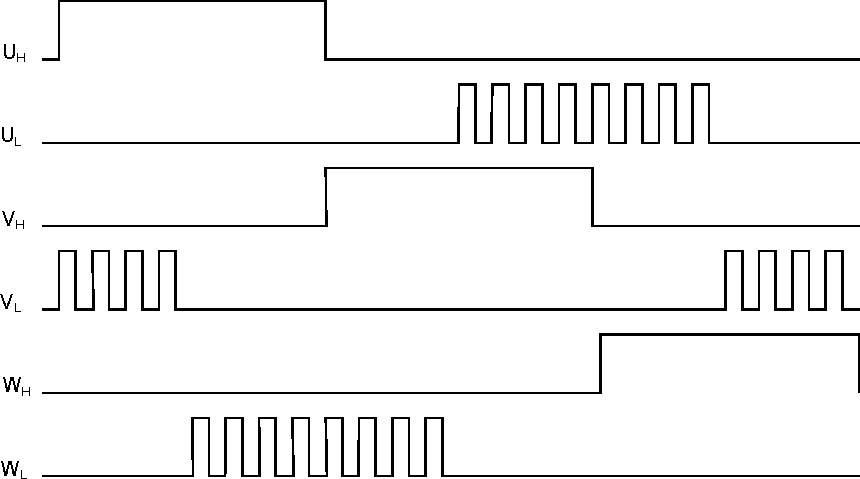
\includegraphics[width=0.9\textwidth]{images/bldcpwm.pdf}
\caption{BLDC Mode PWM Output}
\label{fig_PwmBldcMode}
\end{center}
\end{figure}

To instantiate the PWM service in this mode the following function needs to be called.

\begin{lstlisting}
void do_pwm( chanend c_pwm, 
	buffered out port:32 p_pwm[], 
	clock clk);
\end{lstlisting}

\verb=chanend c_pwm= is the channel used to communication with the client side.

\verb=buffered out port:32 p_pwm[]= is an array of 1 bit ports with an array length of 3 that are used for the HI or LO sides of the inverter respectively.

\verb=clock clk= is the clock block that the PWM thread uses for timing output.

\subsection{PWM Client Usage}
The PWM client functions must be operated on the same core as the server. The usage of the client functions in the various operational modes are described below. The following must be included to call the client functions.

\begin{lstlisting}
#include "pwm_cli.h"
\end{lstlisting}

\subsubsection{Inverter Mode}
The only call required to update the PWM values that are currently being output is listed below. It takes only two arguments, the channel to the PWM server and an array of size three containing unsigned integers that must be between 0 and \verb=PWM_MAX_VALUE=.

\begin{lstlisting}
void update_pwm( chanend c, unsigned value[]);
\end{lstlisting}

This function will process the values and pass them to the PWM service thread.

\subsubsection{Simple three channel PWM mode}

See details above for the Inverter Mode.

\subsubsection{Basic BLDC commutation mode}
The basic BLDC commutation mode client operates slightly differently to achieve the waveform shown in figure \ref{fig_PwmBldcMode}. The function call listed below must be utilised. 

Only a single output is active at any one time and this channel must be identified using the \verb=pwm_chan= argument, this is a value between 0 and 2. The corresponding leg of the inverter needs to be switched manually in the control thread. Please refer to the \verb=app_basic_bldc= application and associated documentation. 

\begin{lstlisting}
void update_pwm( chanend c, 
	unsigned value, 
	unsigned pwm_chan );
\end{lstlisting}

\subsection{PWM Service Implementation}
The PWM service is designed as a continuously running loop that cannot be blocked. This is important to ensure continuous output as stalling an output on an inverter in any application could result in serious failure of the appliance that is being driven.

To achieve the behaviour needed the PWM services are all written in assembly language. This is done to achieve a fine grained control over the instruction sequences required to load up the buffers in the ports and also the port timers.

The PWM service pulls the required data for outputting to the ports from a shared memory location. This is a `double buffered' scheme where the client will update the memory area that is not currently in use and then inform the service via a channel which memory location it should look at for the output data. The update sequence is looked at in more detail in the discussion of the client implementation.

Operation of the full inverter mode is the most complex, so this will be the case that is dealt with here. The other modes (simple three channel and BLDC commutation) are derived from this inverter implementation and thus do not need separate explanation.

We will therefore be covering the operation that is found in \newline \verb=module_dsc_pwm/src/dsc/pwm_svr/inv_svr/=. 

\subsubsection{PWM service port initialisation (pwm\_service\_inv.xc)}
This file achieves a number of functions. The primary function is a wrapper that is called to start the PWM service running. This configures the port and then enters the main loop for the PWM service.

\begin{lstlisting}
#if LOCK_ADC_TO_PWM
void do_pwm_inv( chanend c_pwm, 
    chanend c_adc_trig, 
    in port dummy_port, 
    buffered out port:32 p_pwm[], 
    buffered out port:32 p_pwm_inv[], 
    clock clk)
#else
void do_pwm_inv( chanend c_pwm, 
    buffered out port:32 p_pwm[],  
    buffered out port:32 p_pwm_inv[], 
    clock clk)
#endif
{

  t_out_data pwm_out_data0, pwm_out_data1, pwm_out_data2;
  unsigned buf;

  /* configure the ports */
#if LOCK_ADC_TO_PWM
  // has a dummy port for ADC config
  do_pwm_port_config_inv_adc_trig( dummy_port, 
                                   p_pwm, p_pwm_inv, clk );
#else
  do_pwm_port_config_inv( p_pwm, p_pwm_inv, clk);
#endif

  /* wait for initial update */
  c_pwm :> buf;

  while (1)
  {
  #if LOCK_ADC_TO_PWM
    buf = pwm_op_inv( buf, p_pwm, p_pwm_inv, c_pwm, 
                      c_adc_trig, dummy_port );
  #else
    buf = pwm_op_inv( buf, p_pwm, p_pwm_inv, c_pwm );
  #endif
  }

}
#endif
\end{lstlisting}

The first function calls are the initial configuration of the ports. This is done in \verb=do_pwm_port_config_inv( ... )= or \verb=do_pwm_port_config_inv_adc_trig( ... )= depending on whether the option of ADC triggering has been selected. The function used to configure the ports with the ADC triggering is merely a simple extension of the operation of the mode without ADC triggering and so will be explained here.

\begin{lstlisting}
static void do_pwm_port_config_inv_adc_trig( in port dummy, 
  buffered out port:32 p_pwm[], 
  buffered out port:32 p_pwm_inv[], 
  clock clk )
{
  unsigned i;

  for (i = 0; i < PWM_CHAN_COUNT; i++)
  {
    configure_out_port(p_pwm[i], clk, 0);
    configure_out_port(p_pwm_inv[i], clk, 0);
    set_port_inv(p_pwm_inv[i]);
  }

  /* dummy port used to send ADC trigger */
  configure_in_port(dummy,clk);

  start_clock(clk);
}
\end{lstlisting}

Firstly three legs of the inverter drive are configured to be attached to the clock block and have an initial output of 0. This is deemed to be a safe start-up configuration as all drives are switched off.

Then, in the loop, the `inverted' ports are configured to output the inverse or complementary of the data that is put into the buffers. This means that only a single data set need be maintained and removes the need for inverting the data using the instruction set as this is done by the port logic.

Following the loop that sets up the individual PWM channels is the configuration for the ADC triggering port. This is an input port that is attached to the same clock block as the PWM output ports. An input port that overlaps other in use ports (as described in the usage section above) will not affect their operation. The dummy port is just used for timing synchronisation when signalling the ADC.

Finally the clock block is started.

Once the ports have been configured the output will remain in the initialised state until the thread receives notification from the client thread that data is available in the shared memory for output. It is important to wait for the first client update otherwise there is a risk of output uninitialised data which may damage the drive circuitry.

Once this information is received the main loop is entered.

\subsubsection{PWM service main loop (pwm\_op\_inv.S)}
The operation of the main loop is best described visually as in the flow chart shown in figure \ref{fig_PwmMainLoopFlow}. The entries in the flow chart relate directly to the labels within the main loop. 

A brief overview of each part of the main loop are given below. These should be consulted alongside the comments that reside in the code itself.

\begin{figure}[p]
\begin{center}
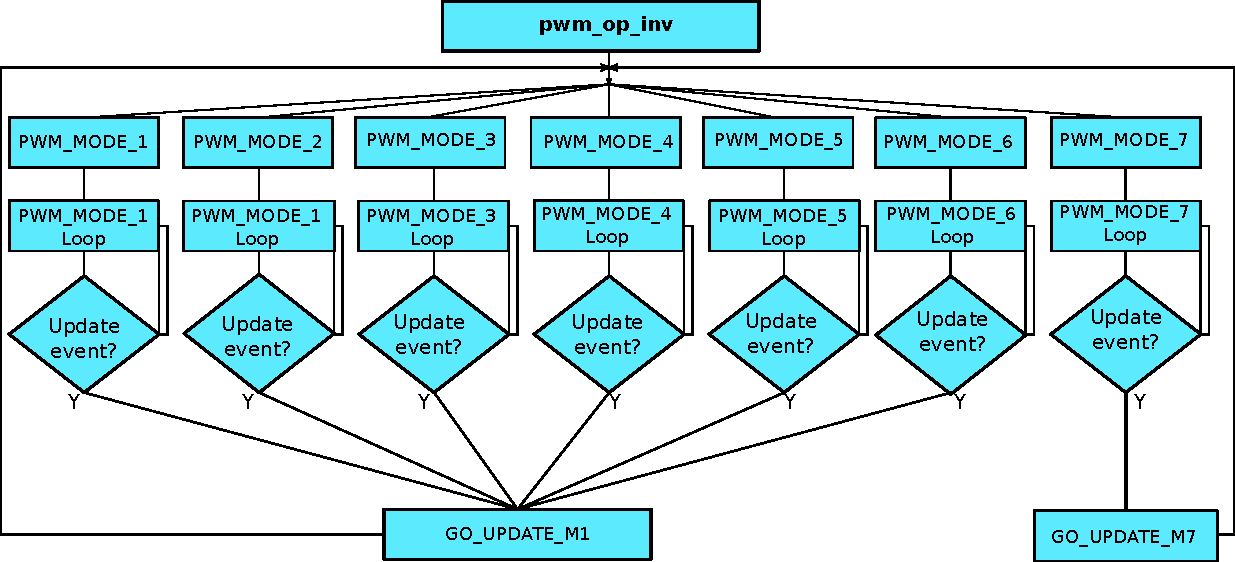
\includegraphics[width=0.9\textheight, angle=90]{images/pwm_loop.pdf}
\caption{PWM Main loop flow chart}
\label{fig_PwmMainLoopFlow}
\end{center}
\end{figure}

The code begins at the \verb=pwm_op_inv= entry point. This begins by running a standard callee save. This preserves any registers that we will clobber as part of the operation of this function. The arguments to the function are then stored on the stack itself in \verb=sp[8:11]=. This ensures we have access to them later.

Following this the registers are moved around into the configuration we require and data is read from the \verb=t_data_out= structure after calculating the appropriate pointers. The port resource IDs are then loaded into registers and the `mode' of operation is read and the port timer read to initialise the synchronisation point.

The code then branches to the appropriate mode according to the mode value that has been read from the data structure provided to it by the client.

\paragraph{Why all these loop modes?} It is worth discussing at this point why there are different loop modes and what they achieve. The nature of the central synchronisation point means that there are very rare times when the edges of the PWM coincide - from an electrical noise standpoint this is beneficial, but from and implementation standpoint it complicates things slightly.

To achieve the required output efficiently using the ports the buffers are used to create the extremely short or long pulses as shown in figure \ref{fig_PwmPortBuffering}. The green boxes indicate a buffer of data that is output from the port.

\begin{figure}[h]
\begin{center}
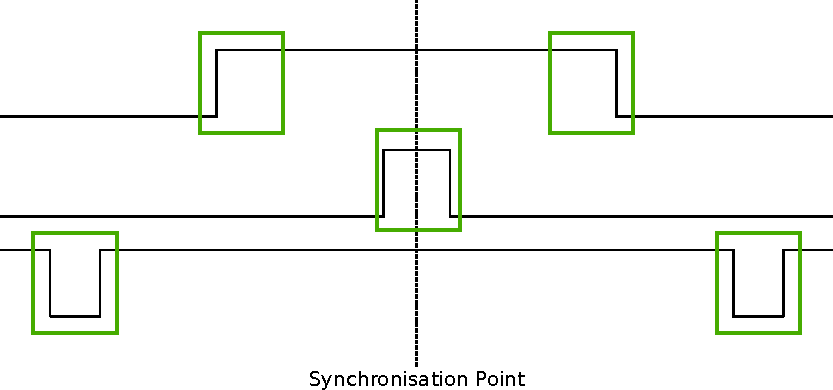
\includegraphics[width=0.9\textwidth]{images/bufferedPWM.pdf}
\caption{PWM Buffered Port Output}
\label{fig_PwmPortBuffering}
\end{center}
\end{figure}

This method of output requires a combination of one or two buffer outputs depending on the length of these pulses. Rather than calculate these during runtime the client will ascertain the particular combination of outputs required and then will define the mode. The different buffering output modes are individually implemented to reduce branching overhead within the loop.

At the entrance to the loop mode (taking \verb=PWM_MODE_4= as the working example) the mode value is replaced with the channel end resource ID. We then enter the core of the PWM service loop. The loop will setup each of the ports in sequence, calculating the appropriate port timer value from the data set that is provided by the client.

When the option to lock the ADC to PWM is required then the system will block on the \verb=in= instruction while it waits for the timer on the dummy port. Once the port timer reaches the required value the thread will output the token to the ADC thread.

If the ADC to PWM lock is not utilised then the thread will pause on the next \verb=setpt= instruction until that particular port timer value is met and the data is output. The ports are loaded in reverse order to turn them off at the correct time. Once all of the channels are reloaded the thread will check for data on the update channel. If data is found then it will immediately enter \verb=GO_UPDATE_M1= otherwise it will continue through the loop calculating the next synchronisation point and looping back to the top of the output sequence.

If the system branches to update then it will execute a sequence very similar to the entry of the function, reading the data out of the data structure and setting up the relevant memory pointers. The update for \verb=PWM_MODE_[1:6]= loops are all the same. In the case of \verb=PWM_MODE_7= the update sequence is slightly different due to the fact that the even is likely to occur when one of the channels is high. This means that a further output is required before receiving the update from the client.

\subsection{PWM Client Implementation}
The PWM client is required to do a number of functions to provide the correct data to the PWM service that outputs the correct values and timings to the ports. The PWM client must:

\begin{itemize}
\item Calculate the output values
\item Calculate the timing values (taking into account dead time)
\item Sort the ports into time order
\item Ascertain the loop mode required
\item Maintain the shared data set, including which buffer is in use and which one can be updated
\end{itemize}

Taking the inverter mode as our working example (located in \newline \verb=module_dsc_pwm/src/dsc_pwm_cli/pwm_cli_inv=) the function \verb=update_pwm(...)= first saves the PWM values for later use and then initialises the channel ordering array to assume a sequential order of output. 

Following this the calculation of the timings and output values are done for each of the channel. This is done by passing the relevant PWM value and data set references to the \verb=calculate_data_out_ref(...)=. This function also ascertains the type of output which can be one of three values \verb=SINGLE=, \verb=DOUBLE= and \verb=LONG_SINGLE=.

Once the calculations for each of the PWM channels is completed they can be ordered. This is done using the \verb=order_pwm(...)= function. This orders the values in the channel ID buffer and also works out the loop mode that is required.

When the values have been ordered and the loop mode calculated the buffer number is passed to the PWM service to indicate an update.


\section{Quadrature Encoder Input}

The quadrature encoder input (QEI) module is provided with a library for both running the thread that handles the direct interface to the pins and also for retrieving and calculating the appropriate information from that thread. 

This module is not explicitly utilised in the current reference design, but could be utilised in the `decoder' thread.

The particular interface that is implemented utilises three signals comprising of two quadrature output (\verb=A= and \verb=B=) and an index output (\verb=I=). \verb=A= and \verb=B= provide incremental information while \verb=I= indicates a return to 0 or origin. The signals \verb=A= and \verb=B= are provided out of phase so that the direction of rotation can be resolved.

\begin{figure}[h]
\begin{center}
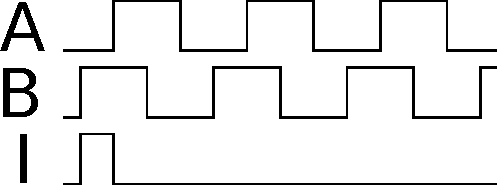
\includegraphics{images/QeiOutput.pdf}
\caption{The quadrature encoder input signals}
\label{fig_QeiInputSignals}
\end{center}
\end{figure}

\subsection{Configuration}

The QEI module requires the following defines in \verb=dsc_config.h=

\begin{lstlisting}
#define QEI_CLIENT_COUNT 2

#define QEI_LINE_COUNT 1024
\end{lstlisting}

The \verb=QEI_CLIENT_COUNT= defines the number of clients that the server supports. This must be a minimum of 1.

The \verb=QEI_LINE_COUNT= defines the number of lines the encoder is specified to have. If this is not defined then 1024 is assumed (as used in the example calculations below). This only affects calculations done by the client functions.

\subsection{QEI Server Usage}
To initiate the service the following include is required as well as the function call shown. This defines the ports that are required to read the interface and the channel that will be utilised by the client thread.

\begin{lstlisting}
#include "qei_server.h"

void do_qei( chanend c_qei[QEI_CLIENT_COUNT],
	port in pQEI);
\end{lstlisting}

\subsection{QEI Client Usage}
To access the information provided by the quadrature encoder the functions listed below can used.

\begin{lstlisting}
#include "qei_client.h"

int get_qei_position( chanend c_qei );

int get_qei_speed( chanend c_qei );

int qei_pos_known( chanend c_qei );

int qei_cw( chanend c_qei );
\end{lstlisting}

Position value is returned in tenths of a degree and speed is returned in revolutions per minute (RPM). 

The third function provides the ability to request whether the QEI interface has received an index signal and is therefore confident that an accurate position can be calculated. Until this function returns 1 then only speed information will be valid.

The fourth function will provide a result of 1 if the direction of rotation of the encoder is clockwise.

\subsection{QEI Service Implementation}
The core functionality is shown below in the state machine in figure \ref{fig_QeiStateMachine}. When in a static state the state machine can be interrupted by a request for rotation data.

\begin{figure}[p]
\begin{center}
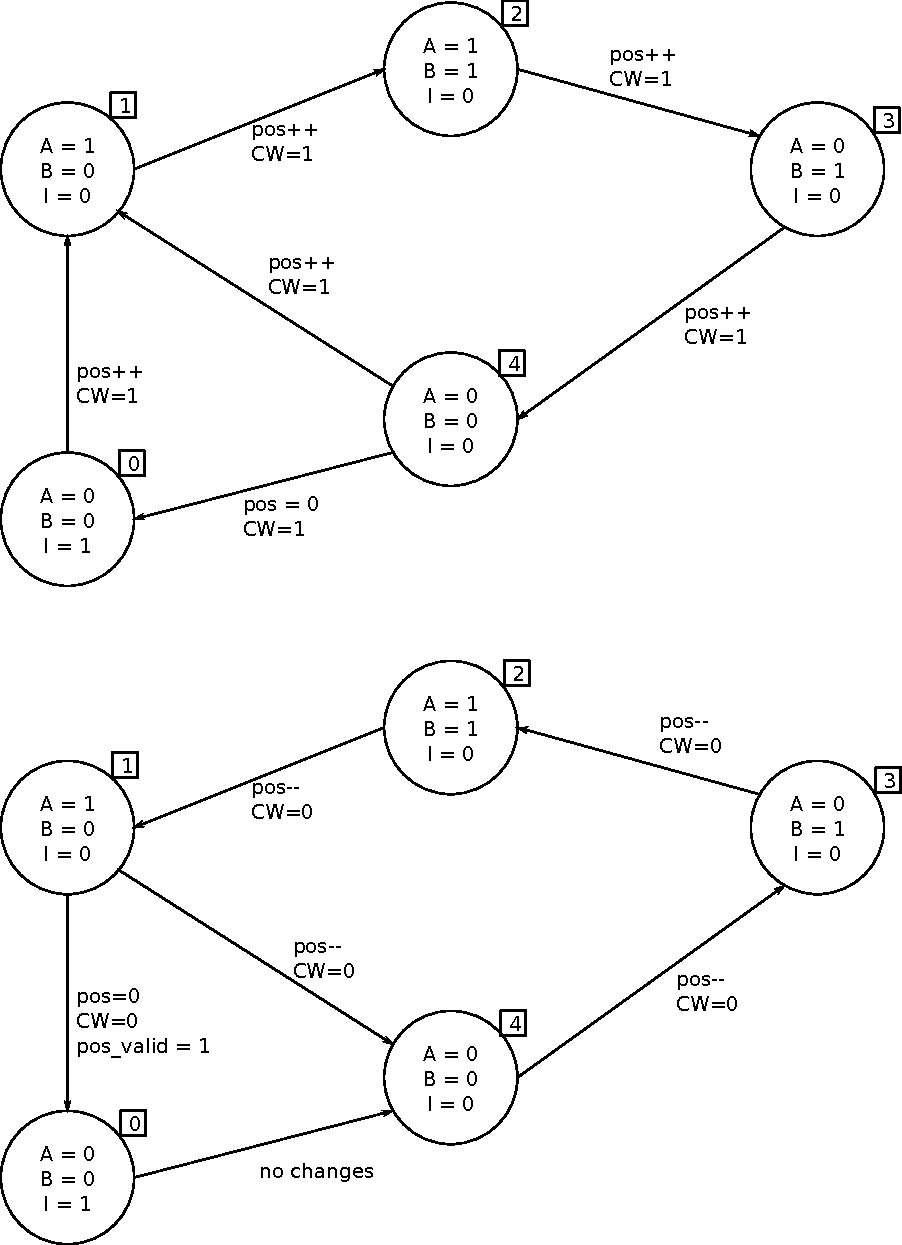
\includegraphics[height=0.9\textheight]{images/qei-state.pdf}
\caption{The QEI state machine showing clockwise and counter clockwise rotation}
\label{fig_QeiStateMachine}
\end{center}
\end{figure}

The request for data will only be served if the event on the channel is enabled. This means that during any state updates the provision of the required data will be a blocked request.

Initialisation of the state machine is done by reading the pins at startup and entering the appropriate state. It is key to note that the position is entirely unknown until an index signal is received, the control algorithm must take account of this. Information as to whether an index value has been received can be queried from the service.

To enable the calculation of both speed and position the time between transitions is recorded and the direction is recorded (as shown for clockwise rotation in the state diagram in figure \ref{fig_QeiStateMachine}).

Communication of the required information is done by the client first requesting the information. This can be requested using the following command values.

\begin{lstlisting}
QEI_CMD_POS_REQ
QEI_CMD_SPEED_REQ
QEI_CMD_POS_KNOWN_REQ
QEI_CMD_CW_REQ
\end{lstlisting}

These are utilised by the client library functions discussed below.

\subsection{QEI Client Implementation}
The client library as described above makes requests to the QEI service thread. These requests are made exclusively via channels and may be blocked during a change in state, but will then be serviced appropriately.

The service thread provides speed and position data in the form of the raw count and time information. This means that to calculate the speed of rotation equation \ref{eqn_QeiSpeed} is utilised on the client side.

\begin{equation}\label{eqn_QeiSpeed}
SPEED =  \frac{60000000}{(t_2 - t_1) \times 1024}
\end{equation}

Calculation of position in tenths of a degree is also performed on the client side and is shown in equation \ref{eqn_QeiPosition}

\begin{equation}\label{eqn_QeiPosition}
POS = (QEI\_RAW\_POS \times 3600) >> 10 
\end{equation}

Direction and whether an index signal has been received are direct values presented as requested from the QEI service.

\section{Analogue to Digital Converter (ADC) Interface}

The analogue to digital interface currently provided is written for the LTC1408. This provides a clocked serial output following a sample and hold conversion trigger signal. The physical interface of the ADC is not covered in detail as the interface for ADC's will vary from manufacturer to manufacturer. An example of the interface for the MAX1379 is also available in this module.

Besides the client and server interfaces the key issue discussed in this section is the synchronisation of the ADC to the PWM and how this is achieved on the ADC side.

\subsection{Configuration}
The define \verb=LOCK_ADC_TO_PWM= must be 0 or 1 for off and on respectively. This defines whether the ADC readings are triggered by the PWM so that measurements can be taken at the appropriate point in the PWM cycle.

\subsection{ADC Server Usage}
The following include and function call are required to operate the ADC software as a server. This server is utilised in the case where the ADC is locked to the PWM.

\begin{lstlisting}
#include "adc_ltc1408.h"

void adc_ltc1408_triggered( chanend c_adc, 
	clock clk, 
	port out SCLK, 
	buffered out port:32 CNVST, 
	in buffered port:32 DATA, 
	chanend c_trig, 
	chanend ?c_logging0, 
	chanend ?c_logging1, 
	chanend ?c_logging2 )
\end{lstlisting}

\verb=chanend c_adc= is the channel where values from the ADC are received.

\verb=clock clk= is the clock block for control data flow to and from the ADC

\verb=port out SCLK=, \verb=buffered out port:32 CNVST= and \verb=in buffered port:32 DATA= are the ports used for interfacing to the ADC.  

\verb=chanend c_trig= is the channel between the PWM and the ADC threads that triggers the conversion of the ADC.

\verb=chanend ?c_logging0=, \verb=chanend ?c_logging1= and \verb=chanend ?c_logging2= are optional channels that can be used to pass data out for logging values.

\subsection{ADC Client Usage}
The functions below are the primary method of collecting ADC data from the ADC service. 

The client can be utilised as follows:

\begin{lstlisting}
#include "adc_client.h"

void do_adc_calibration(chanend c_adc);

{unsigned,unsigned,unsigned} get_adc_vals_raw(chanend c_adc);

{int, int, int} get_adc_vals_calibrated_int16(chanend c_adc);
\end{lstlisting}

\verb=do_adc_calibration(...)= is used to initialise the ADC and calibrate the 0 point. This does an average over 64 ADC readings.

\verb=get_adc_vals_raw(...)= is used to get the raw values from the ADC. In the case of the LTC1408 these are the raw 14 bit values that the ADC delivers. This is a multiple return function in channel order.

\verb=get_adc_vals_calibrated_int16(...)= is used to get the three ADC values with the zero calibration, offset and scaling applied to get a signed 16 bit value. This is a multiple return function in channel order.

There is also an example of an experimental server providing continuous ADC readings that are filtered and provided when requested by the client side.

\subsection{ADC Server Implementation}
The ADC server implementation discussed here is the triggered variant of the ADC code.

The ADC server first configures the ports as clocked inputs and outputs. Following this the main loop is entered. 

ADC readings are triggered by the receipt of a trigger control token over the channel. A token is used as this offers minimum latency for channel communication. Following the token being received the ADC values are read after a time constant that is calibrated to align with the appropriate measurement point.

ADC values can be requested from the server at any point. There are three commands that can be passed indicating whether the client wishes to receive ADC values [0:2], [3:5] or [0:5].

\section{Hall Sensor Interface}
The hall sensor interface is used for measuring speed and estimating the position of the motor. 

\subsection{Hall Sensor Usage}
The hall sensor input module provides a number of functions and options in its usage. A listing of the available functions is given below.

\begin{lstlisting}
#include "hall_input.h"

void run_hall_speed_timed( chanend c_hall, 
	chanend c_speed, 
	port in p_hall, 
	chanend ?c_logging_0, 
	chanend ?c_logging_1 );

void do_hall( unsigned &hall_state, 
	unsigned &cur_pin_state, 
	port in p_hall );
	
select do_hall_select( unsigned &hall_state, 
	unsigned &cur_pin_state, 
	port in p_hall );

void do_hall_test( port in p_hall );
\end{lstlisting}

\verb=run_hall_speed_timed(...)= provides a server thread which measures the time between hall sensor state transitions on a 4 bit port as provided on the motor control platform. This functions implementation is described in more detail below.

\verb=do_hall(...)= simply writes the next hall state into the \verb=hall_state= variable and current pin state into the \verb=cur_pin_state= variable.

\verb=do_hall_select(...)= is the same as \verb=do_hall(...)= but is a \verb=select= function. This function is used in the basic BLDC demonstration application.

\verb=do_hall_test(...)= simply prints out the values received on the hall sensor input port.

\subsection{Hall Sensor Client}
When using the hall sensor server thread as described above, the information may be accessed by using the client functions as listed below.

\begin{lstlisting}
#include "hall_client.h"

{unsigned,unsigned,unsigned} 
	get_hall_pos_speed_delta(chanend c_hall);
\end{lstlisting}

\verb=get_hall_pos_speed_delta(...)= will request and subsequently return the theta, speed and delta values respectively from the hall input server thread. The theta value is an estimated value, speed is in revolutions per minute (RPM) and delta is currently used for debugging purposes.

\subsection{Hall Sensor Server Implementation}
The function \verb=run_hall_speed_timed(...)= provides a thread that handles hall sensor input functions, speed and angle estimations.

This code is currently considered experimental. 

After initialising the ports and initialising the current hall sensor state the code enters a startup phase. This is where an ideal theta value is passed to the client as the motor is not yet actually turning, so no angular estimation can be made. This continues until the hall sensor thread has received two transitions. 

Following the initial startup sequence the hall sensor thread enters the main operational loop. This comprises of a \verb=select= statement that handles either a request for information from the clients, a timeout to detect no rotation or a state transition on hall sensor.

When a new transition is received the new hall state is stored and the current theta base value is updated. This base value is defined as the angular location of the hall sensor within the motor. The system then defines what the next hall sensor state it should wait for will be.

Once the base angle and next state values have been updated the timing calculations are completed to define the speed and angle calculation. Speed calculation is defined by looking for a full mechanical rotation of the motor where it returns to a defined state.

When the thread receives a request for speed and angle information these are calculated and then delivered over the change. The angle estimation is done by considering the time the motor has taken to travel over a hall sensor sector. It assumes that the hall sensor data is requested at a regular time over the sector (which as it is blocked by the PWM it will be in the example FOC implementation).

Once the values are calculated they are provided to the client over the channel.

\section{Processing Blocks}
This module provides a number of standard computation functions that are utilised in motor control. These are outlined below.

\begin{itemize}
\item PID Calculation Routines
\item Clarke \& Park Transforms
\item Sine \& Cosine lookup
\end{itemize}

\subsection{PID Calculation Routines}
The processing blocks module provides the following PID calculation routines. The coefficients are signed 16 bit fixed point.

\begin{lstlisting}
#include "pid_regulator.h"

void init_pid( int Kp, int Ki, int Kd, 
	pid_data *d );

int pid_regulator( int set_point, int actual, 
	pid_data *d );
	
int pid_regulator_delta( int set_point, int actual, 
	pid_data *d );
	
int pid_regulator_delta_cust_error( int error, 
	pid_data *d );
\end{lstlisting}

\verb=init_pid(...)= is used to initialise the \verb=pid_data= structure values with the coefficient values for $Kp$, $Ki$ and $Kd$.

\verb=pid_regulator(...)= does a standard PID calculation using the \verb=set_point= and \verb=actual= values. It calculates the error and applies the PID coefficients and then returns the result. The returned error will be applied to the \verb=set_point= value.

\verb=pid_regulator_delta(...)= does a standard PID calculation using the \verb=set_point= and \verb=actual= values. It calculates the error and applies the PID coefficients and then returns the resulting error.

\verb=pid_regulator_delta_cust_error(...)= does a standard PID calculation using a precalculated error value. It calculates the error and applies the PID coefficients and then returns the resulting error.

\subsection{Clarke \& Park Transforms}
The processing blocks module provides the following Clarke and park transforms. The internal coefficients are all fixed point values.

\begin{lstlisting}
#include "park.h"
void park_transform( int *Id, int *Iq, 
	int I_alpha, int I_beta, unsigned theta );
void inverse_park_transform( int *I_alpha, int *I_beta, 
	int Id, int Iq, unsigned theta );

#include "clarke.h"
void clarke_transform( int *I_alpha, int *I_beta, 
	int Ia, int Ib, int Ic );
void inverse_clarke_transform( int *Ia, int *Ib, int *Ic, 
	int alpha, int beta );
\end{lstlisting}

Each function has the calculation destinations passed as pointers (or references in XC) and the inputs to the calculations are passed as normal arguments.


\subsection{Sine \& Cosine lookup}
The sine and cosine functions are largely provided for use in the Park transforms, but may be used by other functions if required. The sine table provided operate in 0.1 degree steps. The valid range is 0 to 3599.

The lookup functions provided are as follows.

\begin{lstlisting}
#include "sine_cosine.h"

inline long long sine( unsigned deg );
inline long long cosine( unsigned deg );
\end{lstlisting}

\section{SDRAM Interface}
This module provides details on the SDRAM interface used in the XMOS Motor Control Development Platform.

The SDRAM is 256Mbit (32MBytes in size) organised as 4 banks x 8192 rows x 512 columns x 16 bits.
The address structure is: col | (row << log2(SDRAM\_NCOLUMNS)) | (bank << (log2(SDRAM\_NCOLUMNS) + log2(SDRAM\_NROWS))) when addressing SDRAM locations, so for example for a byte-wide SDRAM the address is a byte address.


\subsection{Hardware Interface}

The SDRAM interface is implemented using ports on XCore 0 - it uses 39 pins in total, including:
\begin{itemize}
\item 1 x 16 bit data bus (this is bi-directional).
\item 1 x 15 bit address bus (using a 16-bit port and incorporating the bank signals).
\item 8 x 1-bit ports for control and clock signals.
\end{itemize}


\subsection{Operation}

The SDRAM server which interacts with the hardware is a single thread with a single channel connecting to it.
The function is called from main with a parameter passing a structure containing the appropriate ports. The server\_thread prototype is:

\lstset{breaklines=true}
\begin{lstlisting}
void sdram_server(chanend c_sdram, REFERENCE_PARAM(sdram_interface_t, p))
\end{lstlisting}

During normal operation, the server only logs entries sent to it over the c\_sdram channel.
It writes the log entries into specified addresses and puts the SDRAM into self-refresh mode when not in use.
Writes are short bursts of ``N`` 32-bit words, ``N`` being a compile time option.
In the current DSC implementation N is 32, making each log entry 128 bytes.

When the entries require reading from the SDRAM, a read operation is performed which returns all the data from the SDRAM.

The implementation operates on 128-byte buffer chunks so that client does not stall the SDRAM inside an I/O loop.
Self refresh mode is entered between chunks to allow the client to take unlimited time to process data.
When in this mode, the SDRAM automatically refreshes the data at the required time interval without intervention from the XCore, to prevent data corruption in the memory.
Note that during debug interrupts (e.g. calls to print.h) the I/O loop may be interrupted, which can in turn corrupt the data if the SDRAM is not in self refresh mode.

When reading the SDRAM after a system failure, the SDRAM driver, Ethernet driver, and related parts of the L2 (services core) must stay in a healthy state for the read request to come through and be processed.
Shared memory between these parts and the rest of the system is recommended as a means of decoupling (channels are blocking and therefore not suitable for fault tolerance).


\subsection{Performance}

The expected write bandwidth is 12.5 MB/s.
Read bandwidth is lower, which is OK, as when reading the memory, the time it takes to dump the contents is not critical, provided it is not too long.

Log entries are received, written into SRAM and then copied from SRAM into SDRAM.
This reduces link utilisation and brings overall data rate down to less than a half of the 12.5 MB/s bandwidth.


\subsection{Interface}

This details the client interface that other threads must use to read to and write from the SDRAM. c\_sdram is the channel to the sdram\_server(...).


\subsection{Client Usage}
Before using the client interface, following is required to be included.

\begin{lstlisting}
#include "dsc_sdram.h"
\end{lstlisting}


\subsubsection{Write a packet}

\begin{lstlisting}
c_sdram <: 1;
master
{
	c_sdram <: address;

	for (i = 0; i < SDRAM_PACKET_NWORDS; i++)
	{
		c_sdram <: packet[i];
	}
}
\end{lstlisting}


\subsubsection{Read all SDRAM contents}

\begin{lstlisting}
c_sdram <: 2;

for (i = 0; i < SDRAM_NWORDS; i++)
{
	c_sdram :> word;
}
\end{lstlisting}
\section{Display \& Shared IO Interface}
This module provides a details on the display interface and shared IO manager used in the XMOS Motor Control Development Platform.

The shared IO manager interfaces to the following components on the board:

\begin{itemize}
\item A Newhaven Display NHD-C12832A1Z-FSW-FBW-3V3 128 x 32 pixel monochrome LCD display via a SPI like interface.
\item Ethernet reset signal.
\item CAN PHY control signals (TERM and RS).
\item The 4 push button surface mount switches (marked A-D).
\end{itemize}

Provision could also be made in this thread to drive the 4 surface mount LEDs next to switches A-D.


\subsection{Hardware Interface}

The interface is implemented using ports on XCore 1 - it uses 11 pins in total, including:

\begin{itemize}
\item 1 x 4 bit port shared between the Ethernet reset, CAN control and display address / data signals.
\item 3 x 1-bit ports for the display chip select, serial clock and data signals.
\item 4 x 1-bit ports for the buttons A-D. 
\end{itemize}


\subsection{Operation}

The following files are used for the display and shared IO manager.

\begin{itemize}
\item lcd.h - prototypes for LCD functions
\item lcd.xc - LCD driver functions
\item lcd\_data.h - contains the lcd driver font map.
\item LCD\_logo.h - contains the XMOS logo as a unsigned char array.
\item shared\_io.h - header for the  main shared IO server and defines commands this thread uses.
\item shared\_io.xc - contains the main shared IO server routine. 
\end{itemize}

The shared IO manager that interacts with the hardware is a single thread with three channels connecting to it.
The function is called from main with parameters passing a structure containing the appropriate ports into it.
The server\_thread prototype is:

\tiny
\lstset{breaklines=true}
\begin{lstlisting}
void display_shared_io_manager( chanend c_eth, chanend c_can, chanend c_control, REFERENCE_PARAM(lcd_interface_t, p), in port btns[] )
\end{lstlisting}

The input channels are used for the following communications:

\begin{itemize}
\item c\_eth - receives Ethernet reset signals from the Ethernet MAC.
\item c\_can - receives changes for the CAN control signals from the CAN PHY.
\item c\_control - receives speed and current information from the main motor control thread and sets the speed requested.
\end{itemize}

The main shared IO manager is constructed from a select statement that sits inside a while(1) loop, so that it gets executed repeatedly.

\begin{itemize}
\item \verb!case t when timerafter(time + 10000000) :> time :! - timer that executes at 10Hz. This gets the current speed, current Iq and speed setpoint from the outer motor speed control loop and updates the display with the new values. It also debounces the buttons.
\item \verb!case c_eth :> eth_command :! - receives Ethernet reset signals from the Ethernet MAC and sets/unsets the appropriate bit.
\item \verb!case c_can :> can_command :! - receives changes for the CAN control signals from the CAN PHY and sets/unsets the appropriate bits.
\item \verb"case !btn_en[0] => btns[0] when pinseq(0) :> void :" - execute commands if button A is pressed. Increases the desired speed by PWM\_INC\_DEC\_VAL and sends it to the outer motor speed control loop.
\item \verb"case !btn_en[1] => btns[1] when pinseq(0) :> void :" - execute commands if button B is pressed. Decreases the desired speed by PWM\_INC\_DEC\_VAL and sends it to the outer motor speed control loop.
\item \verb"case !btn_en[2] => btns[2] when pinseq(0) :> void :" - execute commands if button C is pressed. No actual command is executed.
\item \verb"case !btn_en[3] => btns[3] when pinseq(0) :> void :" - execute commands if button D is pressed. No actual command is executed.
\end{itemize}

The switches are debounced by incrementing the but\_en guard signal for that switch by 4 each time they are pressed.
This prevents the code for this button being run until the guard has reached 0.
The 10Hz timer in the select statement decrements the value by one, if the value is not 0, on each iteration though it's loop.
Therefore, after a minimum of 300ms and a maximum of 400ms the switch is re-enabled.


\subsection{LCD Communication}

Communication with the LCD is done using a lcd\_byte\_out(...) function.
This communicates directly with the ports to the display.
The protocol is unidirectional SPI with a separate command / data pin which specifies if the current data transfer is a command or data word.

The procedure for sending a byte to the display is:

\begin{itemize}
\item Select the display using the CS\_N signal.
\item Set the address / data flag (this requires knowing the current port\_val as it is on the shared port).
\item Clock out the 8 bits of data MSB first by:
\item - Setting the data pin to the bit value.
\item - Setting clock high.
\item - Setting clock low.
\item Deselect the display using the CS\_N signal.
\end{itemize}

The following functions are provided that use the lcd\_byte\_out(..) function to send data to the display:

\begin{itemize}
\item lcd\_clear(..) - this wipes the display by writing blank characters into the displays output buffer.
\item lcd\_draw\_image(..) - this takes an unsigned char array of size 512 bytes and writes it to the display. Hence, it can be used to display images on the display.
\item lcd\_draw\_text\_row(..) - writes a row of 21 characters to the display on the row specified by lcd\_row (0-3).
\end{itemize}

The display is configured as 128 columns x 4 byte rows, as the byte writes the data to 8 pixel rows in one transfer.
A 5x7 pixel font map is provided for the characters A-z, a-z, 0-9 and standard punctuation.

The command set for the display is defined in the datasheet.
When sending data to the display it is best to try to send the data as fast as possible.
This is because the display has to be turned off, whilst the data is being written to it.
Therefore, writing large amounts of data on a regular basis can cause the display to flicker.

\section{Low Level Communications Interfaces}
This module provides a details on the low level (typically OSI levels 1-3) interfaces used in the XMOS Motor Control Development Platform.

\subsection{Ethernet Interface}

\subsection{MAC Layer}
The very low level Ethernet interface on the Motor Control Development Platform is implemented using the standard XMOS Ethernet MII and MAC software component.
The hardware interface is implemented using a SMSC LAN8710A 10/100 Ethernet MII PHY.

The original Ethernet component has been edited so that it uses a channel to signal that the reset of the MII PHY is required, rather than signaling it over a actual pin.
The shared IO manager takes this channel and controls the appropriate pin of a shared 4-bit port.

The MAC address is programmed into the OTP of all XCores on the Motor Control Development Platform, in the form 00:22:97:00:4X:XX, where X:XX are the last 3 digits of the serial number encoded as hexadecimal.

Further details will not be included as this software component is documented elsewhere.


\subsection{TCP/IP}

The middle layer of the Ethernet interface is the standard XMOS TCP/IP, which is a port of the open-source uIP TCP/IP stack designed for microcontrollers.
It features a small memory footprint, whilst at the same time enabling high data throughputs if used correctly.
As it only has a sliding window size of 1, the data rate when talking to Windows based PCs can be very low due to the use of delayed ACKs.
The connection must be shutdown and re-establish each time or ACKs must be forced by sending packets back to the board to prevent this problem.

The TCP/IP stack runs on XCore 0, where there is plenty of available MIPS and memory.
It is called from main via a wrapper function that either sets the IP address of the board or configures the TCP/IP stack to use DHCP.
This is controlled by the USE\_DHCP define.


\subsection{CAN Interface}

The CAN Medium Access Control (MAC) interface to the bus is provided by the XMOS CAN software component thread on XCore 1.
The physical (PHY) interface for the CAN bus is provided by a Maxim MAX3059 CAN transceiver.

The MAC also implements the Logical Link Control (LLC) sublayer of the CAN bus, handles errors, as well as providing functions to send and receive packets on the bus.
Bit errors, stuffing errors, form errors and CRC errors are all detected.
All invalid packets are simply discarded when received.
Errors on transmission cause it to retry the transmission.

For the maximum possible throughput of 1Mbps the thread requires 100MIPS of processing, but due to the 7 other threads running on this core this is not possible.
The thread gets a maximum of 62.5MIPS and can therefore run the bus at 500Kbps.
The CAN baud rate is set by setting the define "BAUD\_RATE" in CanIncludes.h header file to the required rate in bits per second.

Separate channels are provided for the client to send and receive communications on the CAN interface. 
The prototype for the CAN MAC is provided below:

\begin{lstlisting}
void canPhyRxTx(chanend rxChan, chanend txChan, clock clk, buffered in port:32 canRx, port canTx);
\end{lstlisting}


\subsubsection{Client Interface}

The following functions are available to a client thread to allow it to interact with the CAN MAC:

\begin{itemize}
\item sendPacket(chanend c, struct CanPacket \&p) - non-blocking call to send a packet on the bus.
\item receivePacket(chanend c, struct CanPacket \&p) - blocking call to receive a packet from the bus.
\item printPacket(struct CanPacket \&p) - prints a packet out on the debug interface.
\item initPacket(struct CanPacket \&p) - initiates a packet.
\item randomizePacket(struct CanPacket \&p, int bitZero) - fills a packet with random data.
\end{itemize}

\section{Application Level Communications Interfaces}

This module provides a details on the higher application level communication interfaces used in the XMOS Motor Control Development Platform.
The figure below shows the main threads that are used.

\begin{figure}[h]
\begin{center}
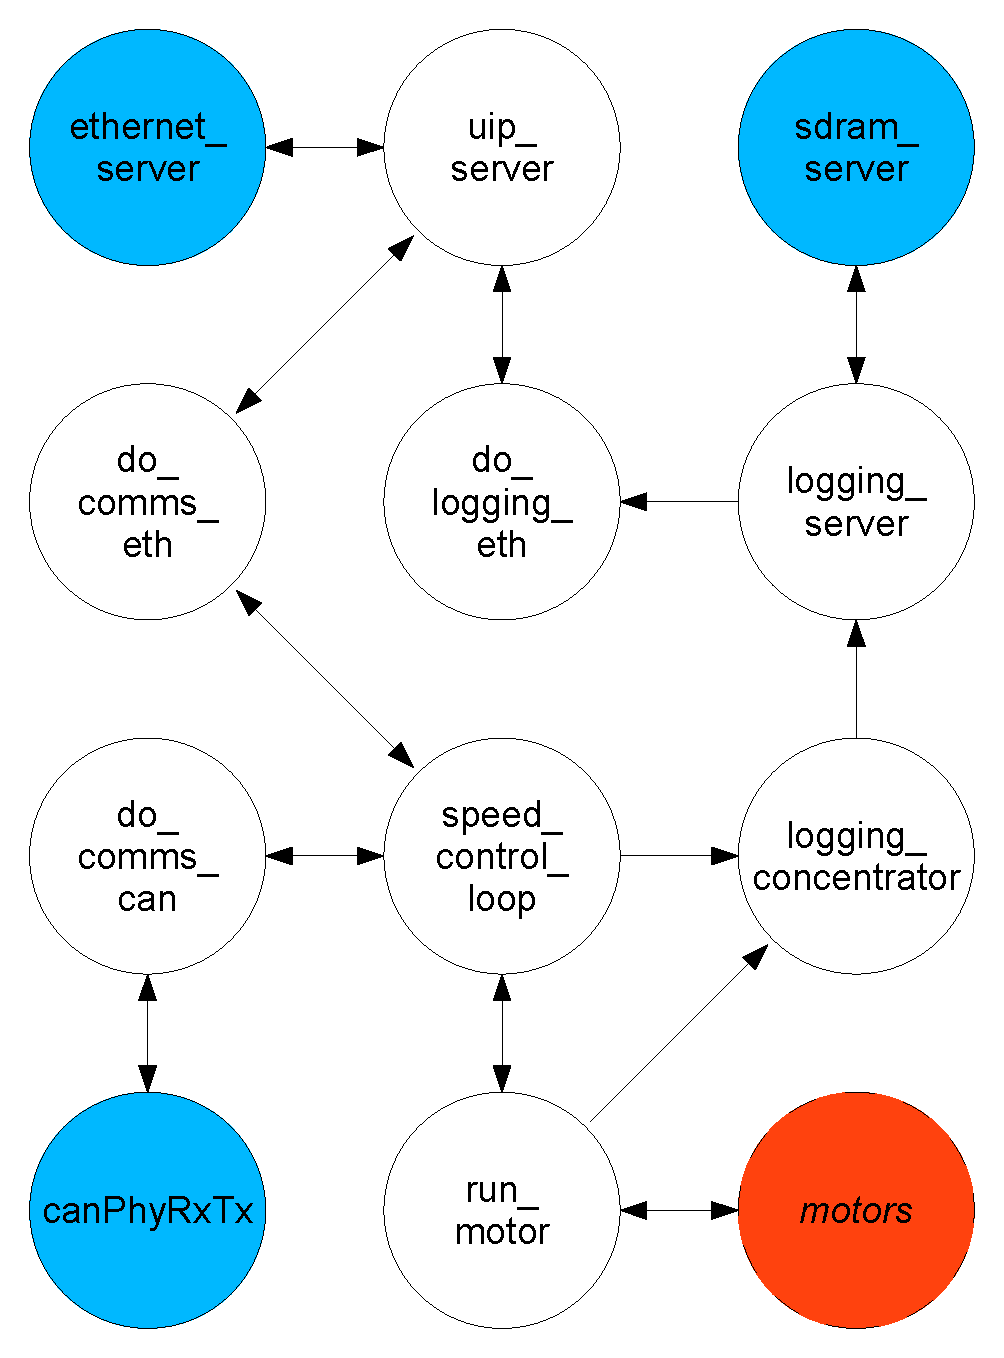
\includegraphics[height=0.6\textheight]{images/comms_threads}
\caption{Communications Thread Diagram}
\label{fig_comms_threads}
\end{center}
\end{figure}

The ethernet\_server and uip\_server threads are the Ethernet and TCP/IP interface, as detailed in the previous section.
The speed\_control\_loop and run\_motor threads are the outer and inner control loops for the motors.
The sdram\_server and canPhyRxTx are the SDRAM and CAN interfaces respectively, as previously discussed.


\subsection{do\_comms\_eth}

The thread do\_comms\_eth interfaces to the TCP/IP stack and provides a server interface on the TCP port defined by TCP\_CONTROL\_PORT (this is typically defined as 9595).

After configuring the TCP port and TCP/IP stack interface, the thread just sits in a \verb!while(1){}! loop processing TCP/IP events. 
The following actions are performed based on the event type:

\begin{itemize}
\item \verb!XTCP_NEW_CONNECTION! - Prints the IP address that the connection is from to the debug output.
\item \verb!XTCP_RECV_DATA! - Main processing function, described below.
\item \verb!XTCP_SENT_DATA! - Closes the send request by sending a 0 byte packet.
\item \verb!XTCP_REQUEST_DATA / XTCP_RESEND_DATA! - Sends the data generated during the \verb!XTCP_RECV_DATA! event to the client.
\item \verb!XTCP_CLOSED! - Closes the connection and prints the IP address that the connection was from to the debug output.
\end{itemize}

The main processing function, receives a packet from the client and processes it according to the criteria below: 

\begin{itemize}
\item if the packets starts "go" then this signals a new connection and nothing is done.
\item if the packets starts "set" then the next four little-endian ordered bytes are converted into the desired speed and sent to the speed\_control\_loop thread.
\item if the packets starts "speed" then the current and desired speeds from the speed\_control\_loop thread are placed in little-endian order into a packet of length 8 bytes and flagged to be returned to the client.
\item if the packets starts "stop" then the connection is closed.
\end{itemize}

The files for this thread are in:

\begin{itemize}
\item \verb!control_comms_eth.xc!
\item \verb!control_comms_eth.h!
\end{itemize}


\subsection{do\_logging\_eth}

The thread do\_logging\_eth interfaces to the TCP/IP stack and provides a server interface on the TCP port defined by TCP\_LOGGING\_PORT (this is typically defined as 9596).

After configuring the TCP port and the TCP/IP stack interface, the thread just sits in a \verb!while(1){}! loop processing TCP/IP events. 
The following actions are performed based on the event type:

\begin{itemize}
\item \verb!XTCP_NEW_CONNECTION! - Prints the IP address that the connection is from to the debug output.
\item \verb!XTCP_RECV_DATA! - Main processing function, described below.
\item \verb!XTCP_SENT_DATA! - Closes the send request by sending a 0 byte packet.
\item \verb!XTCP_REQUEST_DATA / XTCP_RESEND_DATA! - Sends the data generated during the \verb!XTCP_RECV_DATA! event to the client.
\item \verb!XTCP_CLOSED! - Closes the connection and prints the IP address that the connection was from to the debug output.
\end{itemize}

The main processing function, receives a packet from the client and processes it accordingly.
If the packets starts "go" then this signals a request for all the logging data in memory.
The thread then requests the data from the logging\_server thread in 4 byte chunks.
Once 1024 bytes has been received, the thread sends it to the client.

Alternatively, if the packet starts 'A', then this signals an acknowledgement from the host that the data was received and new data can be sent.
This is to force a packet to be generated, to mask the windows delayed ACK problem.
The thread then requests the next 1024 bytes of data from the logging\_server thread in 4 byte chunks, and sends it to the client.
No explicit command is given to signal the end of the data transmission.
The client will receive all data in the SDRAM, provided that every packet is acknowledged.

The files for this thread are in:

\begin{itemize}
\item \verb!logging_comms.xc!
\item \verb!logging_comms.h!
\end{itemize}


\subsection{logging\_server}

This thread controls the interface between the data coming for logging, the SDRAM and the Ethernet logging interface.

The basic operation of this thread, is that it sits in a \verb!while(1){}! loop using a select statement and a timer to log the data it receives from the logging\_concentrator to the SDRAM at 20kHz.
It can also receive requests from the do\_logging\_eth thread over a channel, which cause it to read the contents of all the SDRAM from the sdram\_server and send it back to the do\_logging\_eth thread.

The SDRAM is used as a circular buffer, with each data set (referred to as a record) being of SDRAM\_PACKET\_NWORDS in length.
For a length of 32 words (128 bytes) this gives 262144 records, which at 20kHz is 13.1 seconds of data being recorded.

Each record has a unique number as the first word, which is incremented by one for each record.
This allows the buffer to be de-circulated after it has been read.
When the data is read out, the entire contents of the SDRAM are sent over to the client from low to high memory addresses.
The client is then responsible for de-circulating the data.

The files for this thread are in:

\begin{itemize}
\item \verb!logging_if.xc!
\item \verb!logging_if.h!
\end{itemize}


\subsection{logging\_concentrator}

The function of the logging concentrator is to receive the data from each loop iteration of the outer and inner control loops for the motors.
It also decouples between the control loops and the logging\_server to prevent the pausing of one thread from disrupting the operation of the other.

The thread works by having a select sitting in a \verb!while(1){}! loop processing request on 3 different channels.
These channels are from the outer and inner control loops for the motors and the logging\_server respectively.
The data received from the control loops are placed into the relevant place in the current data packet buffer - this is constantly updated as new data comes in.
When the data is requested by the logging\_server the current packet buffer is streamed to this thread, along with a timestamp of when the request was made.
This means that there could be some jitter with the data, as well as some repeated or lost samples due to the data coming in and going out not being synchronised.

The files for this thread are in:

\begin{itemize}
\item \verb!logging_if.xc!
\item \verb!logging_if.h!
\end{itemize}


\subsection{do\_comms\_can}

This thread is similar in operation to the do\_comms\_eth thread, and provides the same interface to the speed\_control\_loop.

It works by configuring the CAN interface and then sitting in a \verb!while(1){}! loop receiving packets from the CAN interface.
Once the thread receives a packet from the client, it looks at the command type, and processes it accordingly.

\begin{itemize}
\item If command type (byte 2) equals 1, then this command sends the current speed and desired speed to the client.
\item If command type (byte 2) equals 2, then this command sets the desired speed from the data supplied in the packet.
\end{itemize}

The format of a received CAN packet is:

\begin{itemize}
\item 2 bytes - sender address - used to address the return packet if required.
\item 1 byte - command type 
\item 4 bytes - desired speed in big-endian order if command equals 2.
\end{itemize}

The format of a transmitted CAN packet is:

\begin{itemize}
\item 4 bytes - current speed in big-endian order.
\item 4 bytes - desired speed in big-endian order.
\end{itemize}

The files for this thread are in:

\begin{itemize}
\item \verb!control_comms_can.xc!
\item \verb!control_comms_can.h!
\end{itemize}



\section{Motor Control Platform Example Applications}
The current release package ships with two example applications.

\begin{itemize}
\item An application showing an example, but non-functioning Field Oriented Control (FOC) control loop (app\_dsc\_demo)
\item An application showing speed control of the provided motor using basic BLDC code (app\_basic\_bldc)
\end{itemize}

\subsection{Basic BLDC Speed Control Application (app\_basic\_demo)}
This applications makes use of the following functionality.

\begin{itemize}
\item PWM
\item Hall Input
\item Display
\item Ethernet \& Communications
\item Processing Blocks
\end{itemize}

\subsubsection{Motor Control Loop}
The main motor control code for this application can be located in \newline \verb=src/motor/run_motor.xc=. The motor control thread is launched using the following function.

\begin{lstlisting}
void run_motor ( chanend c_wd, 
	chanend c_pwm, 
	chanend c_control, 
	port in p_hall, 
	port out p_pwm_lo[] );
\end{lstlisting}

This is in essence an entirely open loop function that bases the commutation upon the current hall sensor state.

After initially pausing and starting the watchdog the main loop is entered. The main loop responds to two events. The first event is a change in hall sensor state. This will trigger an update to the low side of the inverters (\verb=p_pwm_lo=) and also to the PWM side of the inverter based on the hall sensor state. The output states are defined by the lookup arrays declared at the start of the function.

\begin{lstlisting}
/* sequence of low side of bridge */
unsigned bldc_ph_a_lo[6] = {1,1,0,0,0,0};
unsigned bldc_ph_b_lo[6] = {0,0,1,1,0,0};
unsigned bldc_ph_c_lo[6] = {0,0,0,0,1,1};

/* sequence of high side of bridge */
const unsigned bldc_high_seq[6] = {1,2,2,0,0,1};
\end{lstlisting}

The other event that can be responded to is a command from the \verb=c_control= channel. This can take the form of two commands. The first command is a request to read the current speed value. The second command is a request to change the PWM value that is being sent to the PWM thread and subsequently the motor.

\subsubsection{Speed Control Loop}
The speed control loop for this application can be found in \newline
\verb=src/control/speed_control.xc=. The thread is launched by calling the following function.

\begin{lstlisting}
void speed_control(chanend c_control, 
	chanend c_lcd, 
	chanend c_ethernet );
\end{lstlisting}

This thread begins by initialising the PID data structure with the required coefficients. Following this a startup sequence is entered. This triggers open loop control to get the motor to begin rotating. After a sufficient time period the main speed loop is entered into.

The main loop consists of a \verb=select= statement that responds to three events. The first event is a timed event that triggers the PID control and an update to the motor control threads PWM value. This simply applies the calculated PID error to the set point that is requested.

The second and third events are a request from the LCD and buttons thread or the ethernet thread. This can either be a request from the display for updated speed, set point and PWM demand values or a change in set point. 

\subsection{FOC Application (app\_dsc\_demo)}
This applications makes use of the following functionality. The FOC application is given as an example only. It is not currently functional with the motor that is provided.

\begin{itemize}
\item PWM
\item Hall Input
\item ADC
\item Display
\item Ethernet \& Communications
\item Processing Blocks
\item Logging (includes SDRAM)
\end{itemize}

\subsubsection{Current Control Loop}
The inner current control loop can be found in \verb=src/motor/inner_loop.xc=.

The current control loop takes the demand value from the outer loop and applies it via PWM. This utilises the feedback from the ADC and calculations done using the Park and Clarke transforms and application of PID regulation of $I_d$ and $I_q$.  The resulting values of $V_a$, $V_b$ and $V_c$ are output to the PWM.

This loop is a simple of how a control loop may be implemented and the function calls that would be used to achieve this.

\subsubsection{Speed Control Loop}
This speed control loop found in \verb=src/motor/outer_loop.xc= is in many respects the same in operation as the speed control loop used in the basic BLDC demonstration code and much of the explanation above applies to this application. 

The speed control loop implemented in this application does however have the added feature of allowing the developer to apply step response demands to the inner loop for experimentation purposes. This is done on a timer event that counts through a sequence of time periods. For this to work effectively any requests from the ethernet, CAN or buttons should be ignored. 





\clearpage
\finish
